% !TEX encoding = UTF-8
% !TEX TS-program = pdflatex
% !TEX root = ../tesi.tex

%**************************************************************
\chapter{Il progetto di stage}
\label{cap:il progetto di stage}
%**************************************************************

\intro{Brevissima introduzione al capitolo}\\

%**************************************************************
\section{L'idea}

Nei ristoranti sushi moderni quasi tutti applicano la formula "all-you-can-eat", con tale formula i ristoranti offrono la possibilità di ordinare senza limiti ad un prezzo fisso. I consumi dei clienti in questi locali è maggiore rispetto ai ristoranti à la carte, perché con la formula all-you-can-eat spesso i clienti mangiano oltre il loro livello di sazietà, quindi comporterà un elevato numero di ordinazioni da gestire creando così il problema di capire poi chi ha ordinato i piatti singoli nel momento della consegna. L'idea dunque è stata quella di creare una web-app per la gestione delle ordinazione dei piatti.

\section{La soluzione individuata}
SyncLab ha deciso di risolvere questo problema tramite una web-app, essa è composta da due componenti la parte front-end e la parte back-end. La parte di back-end dovrà essere implementata tramite spring, il back-end ha il ruolo pricipale di un web server, il quale ha il compito di comunicare con il data-base, dove verranno salvati tutte le informazioni dei piatti e degli eventuali ordini dei ristoranti. Il web server deve offrire delle API, con le quali la parte front-end, che utilizza Angular, comunicherà con il server. 
\begin{figure}[H]
    \centering
    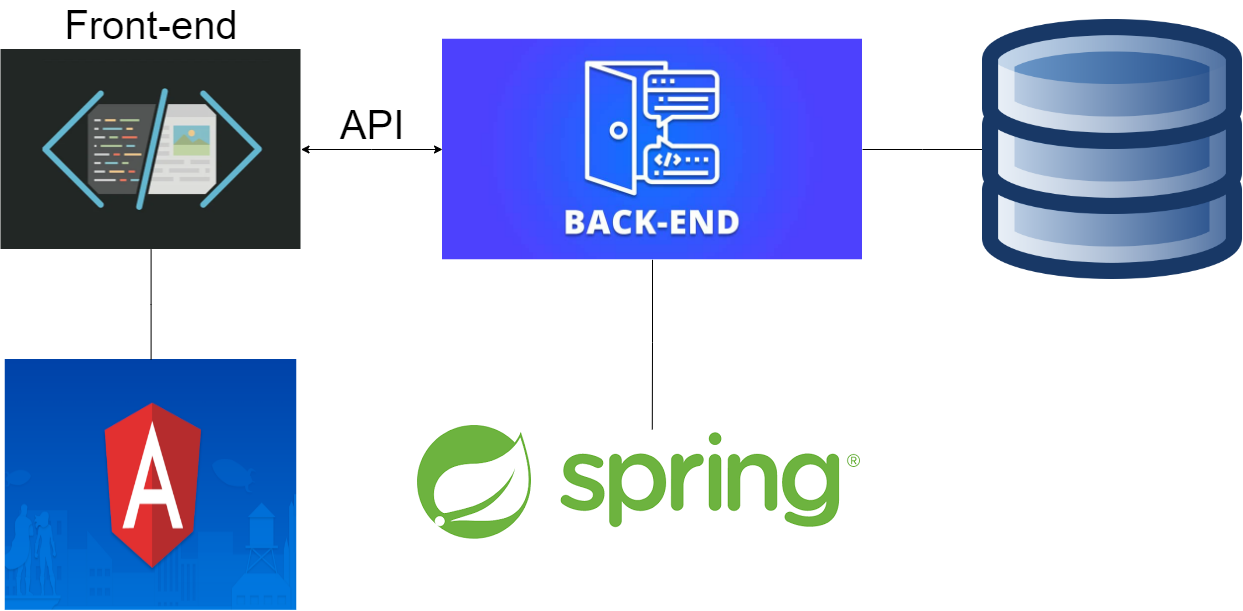
\includegraphics[scale=0.25]{diagramma.png}
    \caption{Diagramma dei componenti per la web-app}
\end{figure}
Angular è un framework open source gratuita per lo sviluppo di applicazione web. Il linguaggio di programmazione utilizzato è TypeScript, TypeScript estende la sintassi di JavaScript, quindi qualsiasi codice scritto in JavaScript è eseguibile anche tramite TypeScript senza nessuna modifica o aggiunta di codice. Grazie a TypeScript il codice generato da Angular gira su tutti i pricipali web browser comuni come Google Chrome, Firefox, Safari, Opera, Microsoft Edge e tanti altri. La web-app, per ciascuna parte dell'applicazione è stata affidata a più persone. Discutendo con il tutor aziendale, Fabio Pallaro, abbiamo individuato i principali obbiettivi per realizzare la web-app ed a me è stato assegnato il compito di sviluppare la visuale dell'applicazione. 

\section{obbiettivi richiesti}
\subsection{Notazione}
Si farà riferimento ai requisiti secondo le seguenti notazioni:
\begin{itemize}
    \item O per i requisiti obbligatori, vincolanti in quanto obiettivo primario richiesto dal committente;
    \item D per i requisiti desiderabili, non vincolanti o strettamente necessari, ma dal riconoscibile valore
    aggiunto;
    \item F per i requisiti facoltativi, rappresentanti valore aggiunto non strettamente competitivo.
\end{itemize}
Le sigle precedentemente indicate saranno seguite da una coppia sequenziale di numeri, identificativo del
requisito.
\subsection{obiettivi fissati}
Si prevede lo svolgimento dei seguenti obiettivi:
\begin{itemize}
    \item Obbligatori:
    \begin{itemize}
        \item O01: Acquisizione competenze sulle tematiche sopra descritte;
        \item O02: Capacità di raggiungere gli obiettivi richiesti in autonomia seguendo il cronoprogramma;
        \item Portare a termine le implementazioni previste con una percentuale di superamento pari al 80\%        
    \end{itemize}
    \item Desiderabili:
     \begin{itemize}
        \item D01: Portare a termine le implementazioni previste con una percentuale di superamento pari al 100\%
     \end{itemize}
     \item Facoltativi:
     \begin{itemize}
        \item F01: Apportare un valore aggiunto al gruppo di lavoro durante le fasi di progettazione delle interfacce.
     \end{itemize}
\end{itemize}
\subsection{Pianificazione del lavoro}
\subsubsection*{Pianificazione settimanale}
\begin{itemize}
    \item Prima Settimana (40 ore)
    \begin{itemize}
        \item Incontro con persone coinvolte nel progetto per discutere i requisiti e le richieste relativamente
        al sistema da sviluppare;
        \item Presentazione strumenti di lavoro per la condivisione del materiale di studio e per la gestione
        dell'avanzamento;
        \item Condivisione scaletta di argomenti;
        \item Ripasso del linguaggio Java SE;
        \item Ripasso concetti Web (Servlet, servizi Rest, Json ecc.).
    \end{itemize}
    \item Seconda Settimana (40 ore)
        \begin{itemize}
            \item Studio principi generali di Spring Core (IOC, Dependency Injection);
            \item Studio SpringBoot;
            \item Studio Spring Data/DataRest.
        \end{itemize}
    \item Terza Settimana (40 ore)
        \begin{itemize}
            \item Ripasso linguaggio Javascript;
            \item Studio del linguaggio TypeScript.
        \end{itemize}
    \item Quarta Settimana (40 ore)
        \begin{itemize}
            \item Studio piattaforma NodeJS e AngularCLI;
            \item Studio framework Angular.
        \end{itemize}
    \item Quinta Settimana (40 ore)
        \begin{itemize}
        \item Analisi e studio del progetto SushiLab;
        \item Progettazione ed implementazione della nuova maschera di accesso.
        \end{itemize}
    \item Sesta Settimana (40 ore)
    \begin{itemize}
        \item Progettazione ed implementazione nuova maschera "Inserimento Ordine e Gestione Tavolo".
    \end{itemize}
    \item Settima Settimana (40 ore)
    \begin{itemize}
        \item Progettazione ed implementazione nuova maschera "Merge Ordini e Visualizzazione Ordine unico".
    \end{itemize}
    \item Ottava Settimana - Conclusione (40 ore)
    \begin{itemize}
        \item Verifica del funzionamento della web-app;
        \item Validazione della web-app;
        \item Termine integrazioni e collaudo finale.
    \end{itemize}
\end{itemize}
\section{Modalità di lavoro}
L'azienda utilizza lo sviluppo agile del software. La modalità agile aiuta a ridurre il rischio di fallimento sviluppando il software in finestre di tempo limitate chiamate iterazioni che, in genere, durano qualche settimana. Ogni iterazione è un piccolo progetto a sé stante e deve contenere tutto ciò che è necessario per rilasciare un piccolo incremento nelle funzionalità del software: pianificazione, analisi dei requisiti, progettazione, implementazione, test e documentazione. Ogni settimana viene effettuato un incontro con il tutor aziendale per discutere dei problemi trovati durante lo sviluppo e il punto di situazione del progetto.
\section{Strumenti di comunicazione}
Per avere una buona comunicazione con l'azienda si è deciso di utilizzare:
\subsubsection{Discord:}
una piattaforma di VoiP\gl{}, messaggistica istantanea e distribuzione deigitale. Su discord gli utenti comunicano con chiamate vocali, video chiamate ed è anche possibile condividere lo schermo.
\begin{figure}[H]
    \centering
    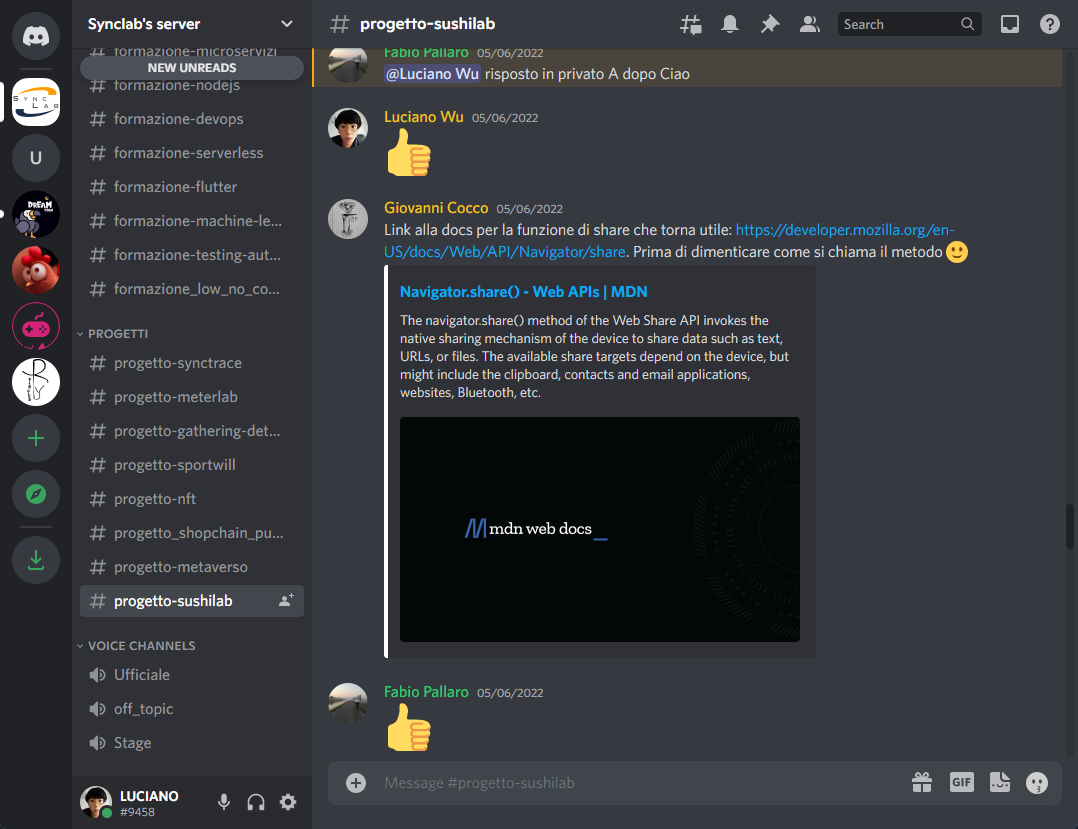
\includegraphics[scale=0.4]{discord.png}
    \caption{Canale SyncLab su Discord}
\end{figure}
\subsubsection{Trello:}
un softwaregestionale in stile Kanban\gl{}, in cui è possibile pianificare il progetto, condividere lo stato di svolgimento di una card con altri collabolatori, spostare vari card tra le liste e assegnare ad un utente.
\begin{figure}[H]
    \centering
    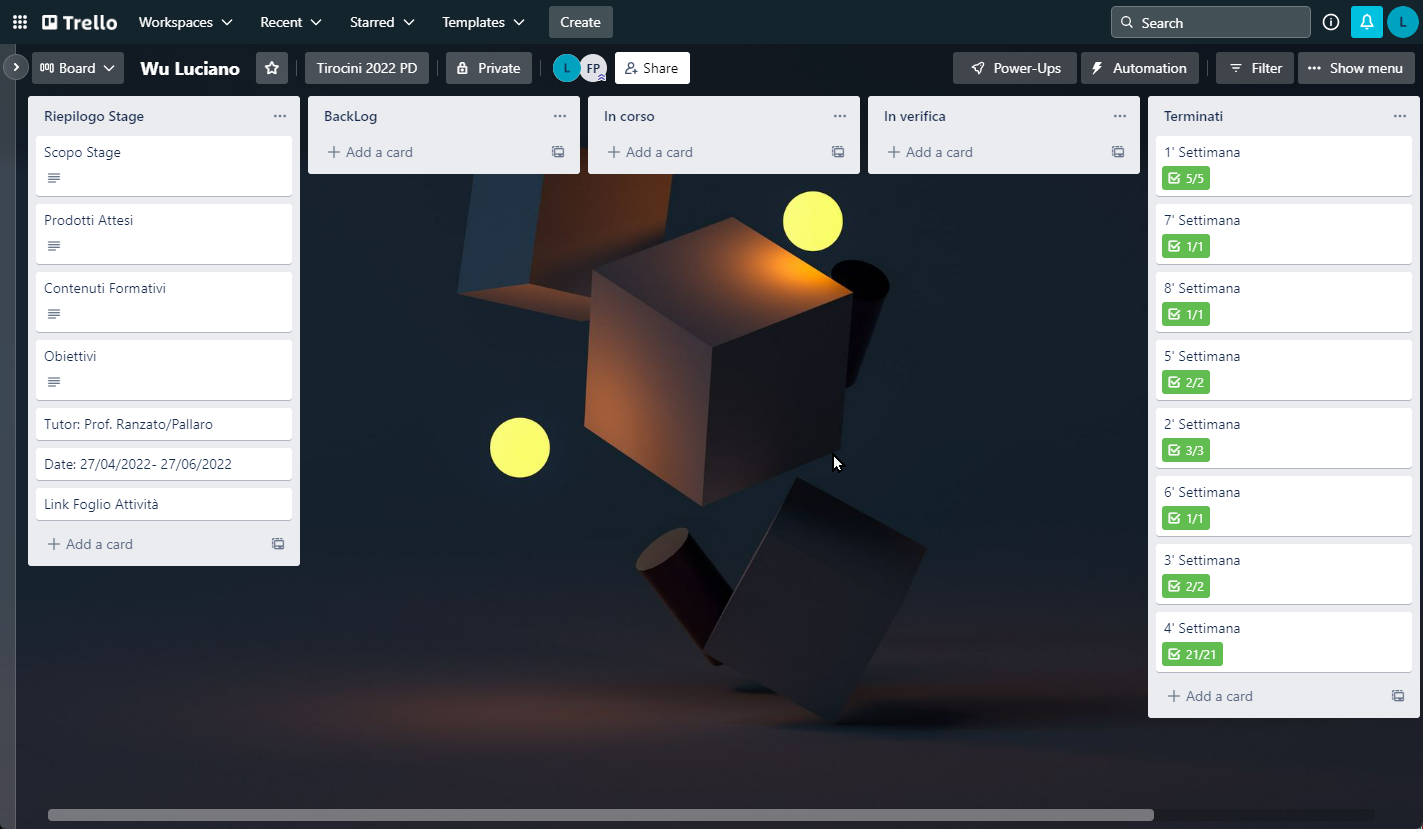
\includegraphics[scale=0.3]{trello.png}
    \caption{Borad di Trello per il progetto sushi-lab}
\end{figure}
\subsubsection{Google Sheets:}
una web-app che fornisce tutte le funzionalità di un foglio elettronico, lo abbiamo utilizzato come un diario giornaliero, dove vengono descritti il compito svolto durante una certa gioranata.
\begin{figure}[H]
    \centering
    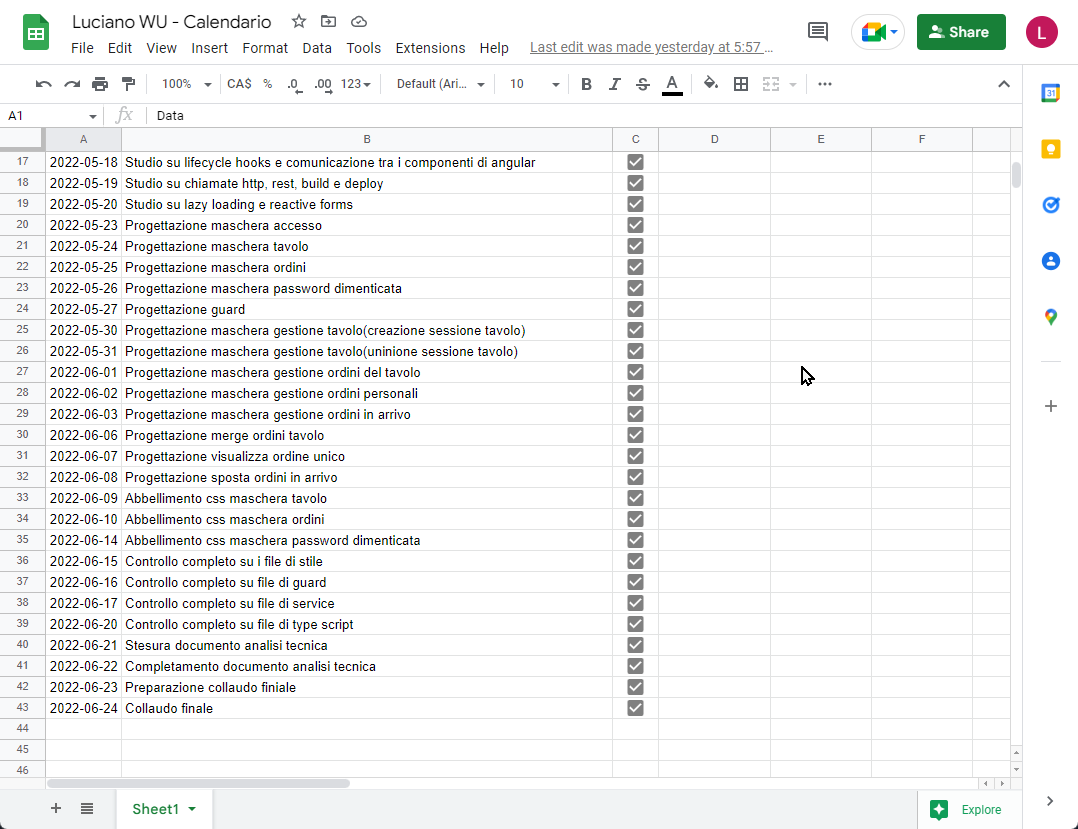
\includegraphics[scale=0.45]{googlesheet.png}
    \caption{Calendario personale per il progetto sushi-lab}
\end{figure}
\subsection{Google Meet:}
un software nata per le videochiamate sviluppato da Goolge, in cui è possibile mandare messaggi e condividere lo schermo e video contemporaneamente, lo abbiamo utilizzato per alcuni incontri con alcuni collabolatori esterni per analisi dei requisiti.
\subsubsection{GitHub:}
servizio di hosting per il sviluppo software, è implementato insieme con lo strumetento di cotrollo versione distribuito Git\gl{}, nel mio caso è utilizzato per condividere e tracciare i file con gli altri collabolatori del progetto.
\begin{figure}[H]
    \centering
    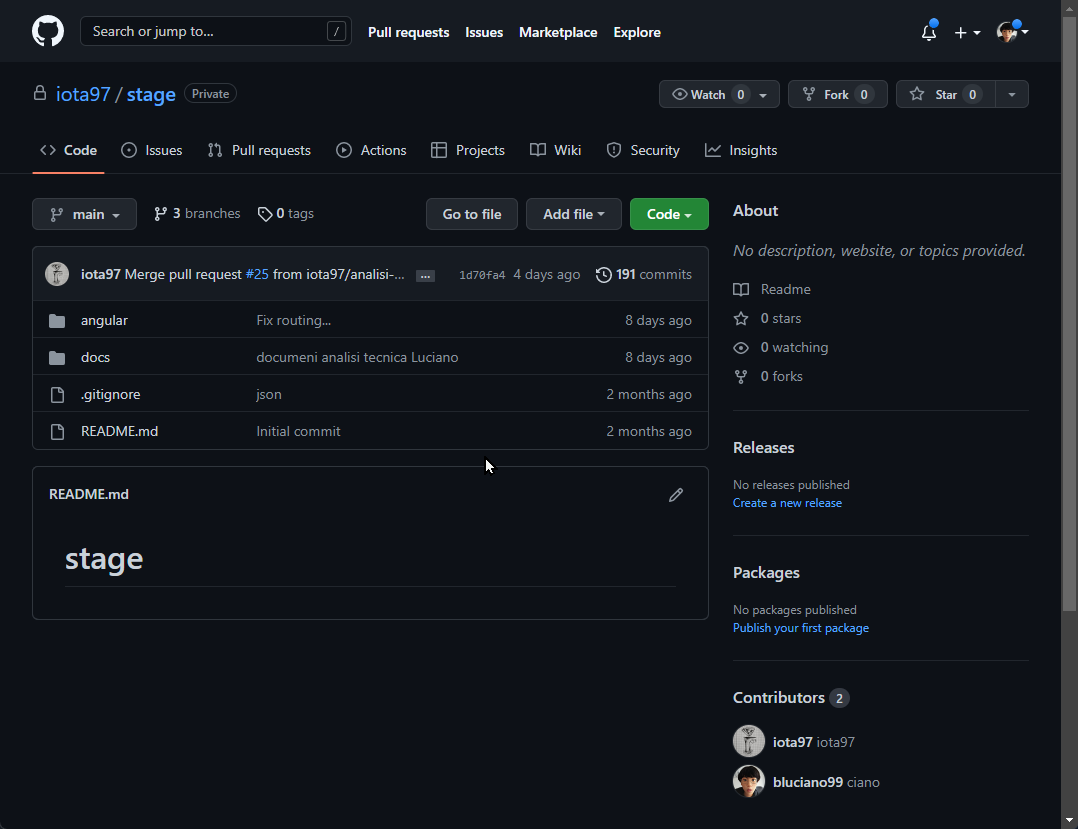
\includegraphics[scale=0.45]{github.png}
    \caption{Repo su GitHub per il progetto sushi-lab}
\end{figure}

% \begin{center}
    
%     \begin{tabular}{ |p{3cm}|p{3cm}|p{3cm}|  }
%         \hline
%         \multicolumn{3}{|c|}{Country List} \\
%         \hline
%         Country Name or Area Name& ISO ALPHA 2 Code &ISO ALPHA 3 \\
%         \hline
%         Afghanistan & AF &AFG \\
%         Aland Islands & AX   & ALA \\
%         Albania &AL & ALB \\
%         Algeria    &DZ & DZA \\
%         American Samoa & AS & ASM \\
% Andorra & AD & AND   \\
% Angola & AO & AGO \\
% \hline
% \end{tabular}
% \end{center}